\subsubsection{Свеска 11}

\zadatak
Реши неједначину
$$
\log_3^2 x - 5\log_3  x + 6 \le 0.
$$

\resenje
Када извршимо смену $t=\log_3 x$, можемо писати да је
$$
t^2-5t+6\le0
$$
Како су решења квадратне једначине\queq\ $t_1=2$ и $t_2=3$,
неједначина је задовољена када је $t\in[2,3]$. \
Пошто је $x=3^t$, следи да је неједначина задовољена за
$x\in[3^2,3^3]$, односно,
$$
\ram{9\le x\le 27}.
$$
\vskip-36pt
$$
\slika{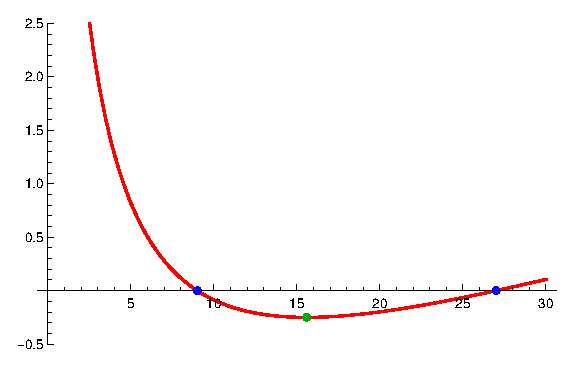
\includegraphics[width=\sirina]{eps/11.eps}}{$y=\log_3^2 x - 5\log_3  x + 6$.}
$$

\dodatak Функција има \idx{минимум} за $t=5/2$, односно, у тачки $(9\sqrt3,-1/4)$.